\documentclass{article}
\usepackage{tikz}
\usetikzlibrary{patterns}
\usepackage{pgfplots}
\begin{document}
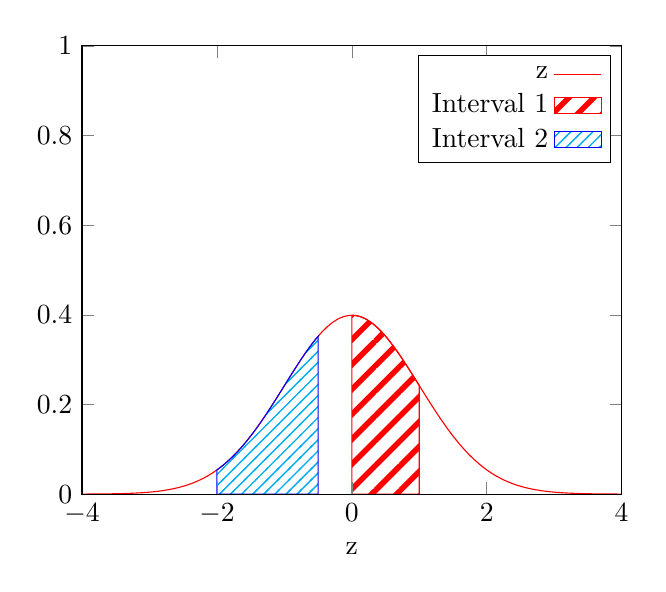
\begin{tikzpicture}
	\tikzset{
		hatch distance/.store in=\hatchdistance,
		hatch distance=10pt,
		hatch thickness/.store in=\hatchthickness,
		hatch thickness=2pt
	}

	\makeatletter
	\pgfdeclarepatternformonly[\hatchdistance,\hatchthickness]{flexible hatch}
	{\pgfqpoint{0pt}{0pt}}
	{\pgfqpoint{\hatchdistance}{\hatchdistance}}
	{\pgfpoint{\hatchdistance-1pt}{\hatchdistance-1pt}}%
	{
		\pgfsetcolor{\tikz@pattern@color}
		\pgfsetlinewidth{\hatchthickness}
		\pgfpathmoveto{\pgfqpoint{0pt}{0pt}}
		\pgfpathlineto{\pgfqpoint{\hatchdistance}{\hatchdistance}}
		\pgfusepath{stroke}
	}
	\makeatother

	\begin{axis}[
			xmin=-4,xmax=4,
			xlabel={z},
			ymin=0,ymax=1,
			axis on top,
			legend style={legend cell align=right,legend plot pos=right}]
		\addplot[color=red,domain=-4:4,samples=100] {1/sqrt(2*pi)*exp(-x^2/2)};
		\addlegendentry{z}
		\addplot+[mark=none,
			domain=0:1,
			samples=100,
			pattern=flexible hatch,
			area legend,
			pattern color=red]{1/sqrt(2*pi)*exp(-x^2/2)} \closedcycle;
		\addlegendentry{Interval 1}
		\addplot+[mark=none,
			domain=-2:-0.5,
			samples=100,
			pattern=flexible hatch,
			hatch distance=5pt,
			hatch thickness=0.5pt,
			draw=blue,
			pattern color=cyan,
			area legend]{1/sqrt(2*pi)*exp(-x^2/2)} \closedcycle;
		\addlegendentry{Interval 2}
	\end{axis}
\end{tikzpicture}
\end{document}
